\chapter{Descripción del trabajo de graduación} \label{chp:01_intro}

\vspace{0.2cm}

El Capítulo 1, titulado "Descripción del Trabajo de Graduación", cumple el papel fundamental de introducción a esta tesis. No solo brinda una visión general del trabajo en sí, sino que también contextualiza su relevancia en el campo de estudio, justificando la elección del tema y resaltando las problemáticas que abordadas a lo largo de la investigación. Asimismo, se establecen de manera clara y precisa los objetivos generales y específicos, trazando el propósito fundamental del estudio y proporcionando una guía para el desarrollo de la investigación. 

\vspace{0.5cm}

En resumen, este capítulo inicial sienta las bases necesarias para comprender el alcance y la importancia del trabajo de graduación que se presenta en la tesis.


\newpage

\section{Introducción} \label{sct:intro:introducción}

El presente tiene como objetivo desarrollar un simulador de trayectoria ascendente y descendente de un globo-sonda, así como el dimensionamiento a subsistema de navegación en misiones de carácter de espacio cercano (Near-Space); aportando significativo a las misiónes Near-Space del Observatorio Micro-Macro (OMM), con un simulador preliminar que desempeña un papel crucial en la mitigación de riesgos y la predicción  de la trayectoria del globo sonda. Además,  esta investigación busca que en el país se avance en el conocimiento de los diferentes factores que influyen en el movimiento de los globos-sonda, lo cual ofrece una mejor comprensión de la exploración de la estratosfera.

En El Salvador,  actualmente lo más cercano relativo al aeroespacio desarrollado es la aviación, remontando su historia a 1885 cuando se dieron los primeros indicios informales, ya en 1929 la aviación se formalizó en el país,  desarrollándose paulatinamente, ver figura \ref{fig:historia}, pero a pesar de estos antecedentes, todavía hay mucho por explorar y desarrollar en el campo aeroespacial \cite{HistoriaACC}. En 2008 se registraron los primeros indicios aeroespaciales y desde entonces se han desarrollado algunos proyectos con esta temática \cite{HistoriaESAI}, \cite{elfaroColibriytorogoz}. En este sentido, resulta indispensable preservar el legado actual, y este trabajo de graduación se presenta como una propuesta que se adhiere a esa misma filosofía. En este contexto, este trabajo se divide en cuatro partes principales: 

\begin{enumerate}
    \item  Se realizó una revisión de precedentes y antecedentes que contextualicen el trabajo.
    \item Se detalla los modelos que componen a la simulación de la trayectoria ascendente y descendente del globo-sonda, donde se exploran las ecuaciones dinámicas, parámetros atmosféricos y geometría \cite{simulador_chino}, \cite{ascentRate_weatherBallon}. 
    \item Se muestra los resultados y se desarrolla un análisis exploratorio de los datos obtenidos de la simulación, el exploratorio fue introductorio y solo se evaluó las medidas de tendencia central y gráficos de las variables.
    \item Con los resultados del exploratorio, se presentó una propuesta de dimensionamiento del subsistema de navegación, dejándose libertad para una  futura fabricación y pruebas de funcionamiento en condiciones similares y reales de la misión aeroespacial.
\end{enumerate}

\begin{figure}[!ht]
    \centering
    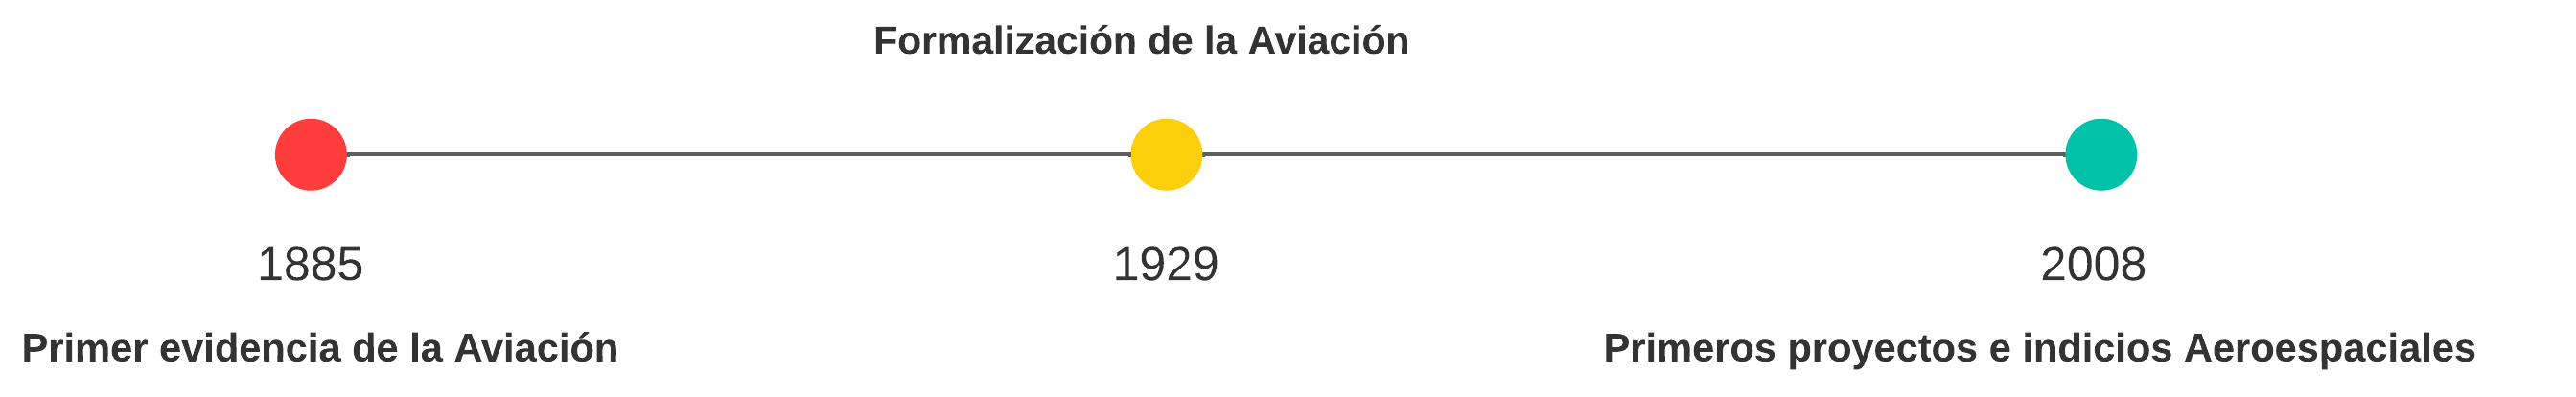
\includegraphics[width=0.85\linewidth]{document/figures/01_linea del tiempo_historia.png}
    \caption{Línea de tiempo de El Salvador, aviación y aeroespacial}
    \label{fig:historia}
\end{figure}

\newpage

\section{Objetivos} \label{sct:intro:objetivos}

\vspace{1.0cm}

\textbf{General}

Desarrollar un modelo de simulación de trayectoria ascendente y descendente de una globo-sonda hasta la estratosfera a través de la selección de diferentes parámetros clave para la misión aeroespacial.

\vspace{1.5cm}

\textbf{Específicos}

\begin{itemize}

    \item[•] Emplear los parámetros simulación que afectan la trayectoria ascendente y descendente de un globo-sonda en la estratosfera, y establecer los parámetros claves que delimiten la simulación.

    \item[•] Simular computacionalmente parámetros clave de un globo-sonda de gran altitud a lo largo de su posible trayectoria, de forma emulen las condiciones.

    \item[•] Desarrollar un análisis exploratorio a partir de los datos que se generaron en la simulación para proporcionar una visión general del equipo necesario para el subsistema de navegación en la misión estratosférica.

    \item[•] Elaborar un dimensionamiento a subsistema de navegación que consista en la selección de componentes electrónicos basándose en el análisis exploratorio realizado, culminando en el desarrollo de esquemático y layout para generar los archivos planteen una futura fabricación.

\end{itemize}

\newpage

\section{Aspectos a considerar} \label{sct:intro:consideraciones}

\subsection{Alcances}

\begin{itemize}

    \item[•] Se plantea el desarrollo de un código fuente capaz de simular la trayectoria dentro de la misión que imiten las condiciones posibles de la misión aeroespacial en la estratosfera, así como la generación de datos de simulaciones para elaborar un análisis exploratorio. 

    \item[•] Proponer un dimensionamiento a subsistema de navegación de bajo costo que incluya los dispositivos necesarios para rastreo de trayectoria y que sean aptos para las condiciones adversas y extremas de la estratosfera basándose en el análisis exploratorio realizado con los datos generados de la simulación.

    \item[•] Proporcionar como producto de este trabajo una herramienta útil para el diseño y la planificación de misiones aeroespaciales similares en el futuro. Ver anexo \ref{chp:anexo:source_thesis}.


\end{itemize} 

\subsection{Limitaciones}

\begin{itemize}

    \item[•] Ningún modelo puede simular y predecir con exactitud y además involucrar todos los parámetros existentes, esto debido a la gran variabilidad de los factores que se pueden encontrarse a lo largo de la trayectoria estratosférica del globo-sonda.

    \item[•] La propuesta de dimensionamiento a subsistema de navegación sólo incluye el desarrollo del esquemático y layout de los circuitos, y también los archivos para una futura fabricación, por lo tanto, excluye la realización de la programación y elaboración en físico de la placa de circuito impreso (PCB). Además, por lo último mencionado, no se realizan pruebas de funcionamiento ni pruebas de exposición de la PCB a las condiciones que emulen los parámetros de las simulaciones del código fuente a realizar.

    \item[•] La selección de componentes en el dimensionamiento del subsistema de navegación está limitada por los recursos disponibles, el alcance y precisión de los sensores; así como también, la disponibilidad y accesibilidad de los componentes electrónicos en el mercado internacional y local.

\end{itemize}

\newpage

\section{Motivación del trabajo} \label{sct:intro:motivacion}

El desarrollo de misiones aeroespaciales como lo serían las estratosféricas plantea un gran desafío, debido a la complejidad de los factores atmosféricos que afectan la trayectoria ascendente y descendente de un globo-sonda, así como los cambios meteorológicos que se presentan a diferentes altitudes que son extremos y cambiantes; es por ello, que es necesario tener una comprensión de las condiciones que se estarán expuestos y realizar simulaciones que modelen una aproximación de las circunstancias posibles de la misión aeroespacial. Con anterioridad, en El Salvador se han desarrollado globos estratosféricos de forma aficionada o en círculos académicos/profesionales \cite{globo_pupuseriasuiza_1},  \cite{globo_nayib_nuevocuscatlan}, \cite{sphere_ESAI}, y existe una constante de hechos comunes que dificultaban el éxito de las misiones de las sondas desarrolladas por ellos, se pueden resaltar algunos: pérdida de equipo, incerteza total o parcial del funcionamiento de la sonda en todo su recorrido y desconocimiento del ambiente/condiciones que podría enfrentar la sonda.

Entonces, es así como este trabajo aborda estos desafíos, proporcionando una solución con el modelamiento de la sonda en su trayectoria para tener una mayor certeza del funcionamiento y situaciones que se enfrenta el equipo y así lograr disminuir costos por perdidas, mitigar riesgos y aumentar las probabilidades de éxito de la misión. Adicional al modelo, se dimensiona un subsistema de navegación que integre una variedad de dispositivos de bajo costo, los más adecuados para las condiciones extremas de la estratosfera y su rastreo/localización;  con el análisis exploratorio se  selecciona los componentes electrónicos y desarrollar el esquemático y layout, generando los archivos necesarios para futura fabricación.

La inspiración para el presente trabajo proviene del proyecto Sphere de ESAI USA y otros proyectos consultados \cite{ sphere_ESAI}, \cite{Irazu_CR}, \cite{pycubed}, ya que no existe ninguna publicación en la región de Centroamericana relacionada con globos meteorológicos o estratosféricos de forma académica, exceptuando usos o aplicaciones comerciales, recreativas y aficionadas documentados en diarios nacionales y publicaciones a lo largo de internet \cite{globo_pupuseriasuiza_1},  \cite{globo_nayib_nuevocuscatlan}, \cite{globo_pupuseriasuiza_2}. Por lo tanto, el presente representa una oportunidad única para explorar y avanzar en esta área de investigación en la región y contribuir a desarrollar subsistemas de navegación de bajo costo para futuras misiones a la estratosfera, así como será beneficioso para futuros investigadores que desean recopilar o procesar datos meteorológicos o con algún otro propósito científico.

\newpage

\section{Contexto del proyecto} \label{sct:intro:contexto}

\subsection{Antecedentes}

Este trabajo tiene sus raíces en el macroproyecto "Diseño de la misión para un globo meteorológico de gran altitud - StratoBalloon", el cual fue creado por el Observatorio Micro Macro (OMM) de la Universidad Don Bosco. Este macroproyecto surgió a partir de la participación de un grupo de estudiantes de ingeniería en el hackathon "Space Apps Challenge 2021" de la NASA \cite{SpaceApps_ASAUDB}, \cite{SpacaApps_noticia_UDB}, donde se logró destacar entre los cinco mejores competidores a nivel nacional. Desde entonces, el equipo ha estado trabajando, llevando a cabo diferentes trabajos de graduación y otras actividades relacionadas con el mismo; uno de los trabajos de graduación realizados hasta la fecha se tituló “Diseño y análisis de un módulo reemplazable para misiones cercanas a la estratosfera (Near-Space LRU)”, desarrollado por Ali Barahona y Manuel Pleites. Este proyecto se enfocó en la parte estructural del macroproyecto y consistió en la realización de impresiones 3D de probetas de ensayo para probar la resistencia mecánica de materiales de impresión, además de realizar diferentes simulaciones mecánicas \cite{tesis_estructura_stratoballoon}.

Se tiene, también que,  "Diseño de la misión para un globo meteorológico de gran altitud - StratoBalloon", es una iniciativa salvadoreña liderada principalmente por un equipo de estudiantes de la Universidad Don Bosco de diversas disciplinas que trabajan juntos para lograr el objetivo de diseñar una misión para un globo meteorológico que pueda ascender a una altitud de 30,000 metros sobre el nivel del mar, con esto se busca obtener una experiencia valiosa en cuanto a liderazgo, trabajo en equipo y habilidades técnicas. El proyecto implica una serie de actividades integradoras para lograr el objetivo que abarcan desde la selección de materiales y equipos necesarios para la misión, hasta el cálculo de trayectorias y la obtención de los permisos legales necesarios para llevar a cabo la misión. 

La misión prevista del macroproyecto abreviada StratoBalloon, ver figura \ref{fig:etapas_mision_stratoballoon},  se desglosa y detalla en las siguientes fases de operación:

\begin{itemize}
    \item \textbf{Fase 1:}  lanzamiento de la sonda desde unas coordenadas predefinidas.
    \item \textbf{Fase 2:} ascenso de la sonda hasta los 30 km.
    \item  \textbf{Fase 3:} explosión del globo, inicia descenso en caída libre.
    \item \textbf{Fase 4:} descenso junto con el paracaídas y la carga útil.
    \item \textbf{Fase 5:}  recuperación de la sonda, fin de la misión.
\end{itemize}

Además,  las fases se pueden dividir en tres: despegue, apogeo y aterrizaje, siendo una versión resumida de las cinco fases presentadas.

\newpage

\begin{figure} [!ht]
    \centering
    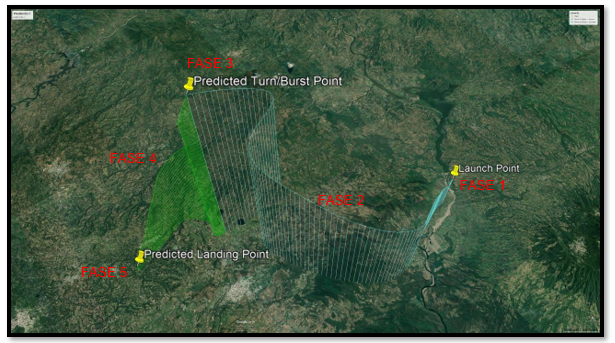
\includegraphics[width=1\linewidth]{document/figures/01_etapas de la mision.png}
    \caption{Etapas de la misión proyectada para StratoBalloon, créditos a \cite{tesis_estructura_stratoballoon}.}
    \label{fig:etapas_mision_stratoballoon}
\end{figure}

Cabe resaltar que en la fase 3 de la operación, véase figura \ref{fig:etapas_mision_stratoballoon}, es donde se alcanza el punto más crítico de la misión para los elementos electrónicos que componen el sistema, pudiendo alcanzar hasta los límites de la estratosfera, siendo afectado por temperaturas extremas, presión casi de vacío, nula densidad atmosférica, aumento de la radiación, humedad, entre otras \cite{nearspaceExperiments}.

En figura \ref{fig:bosquejo_stratoballoon} se muestra el bosque actual desarrollado en StratoBalloon, el cual es un prototipo que aún se está desarrollando y se le van haciendo mejoras a medida el proyecto avanza y se gana experiencia.  En donde se indica '\textit{módulo}' en la figura \ref{fig:bosquejo_stratoballoon},  es el diseño de la estructura actual, en cuyo interior existirán un conjunto de sistemas electrónicos que tienen el propósito de proveer la ubicación espacial, mantener comunicación con una estación en tierra y suministrar y administra la potencia eléctrica entre los demás subsistemas (navegación, telemetría y energía). 


\begin{figure} [!ht]
    \centering
    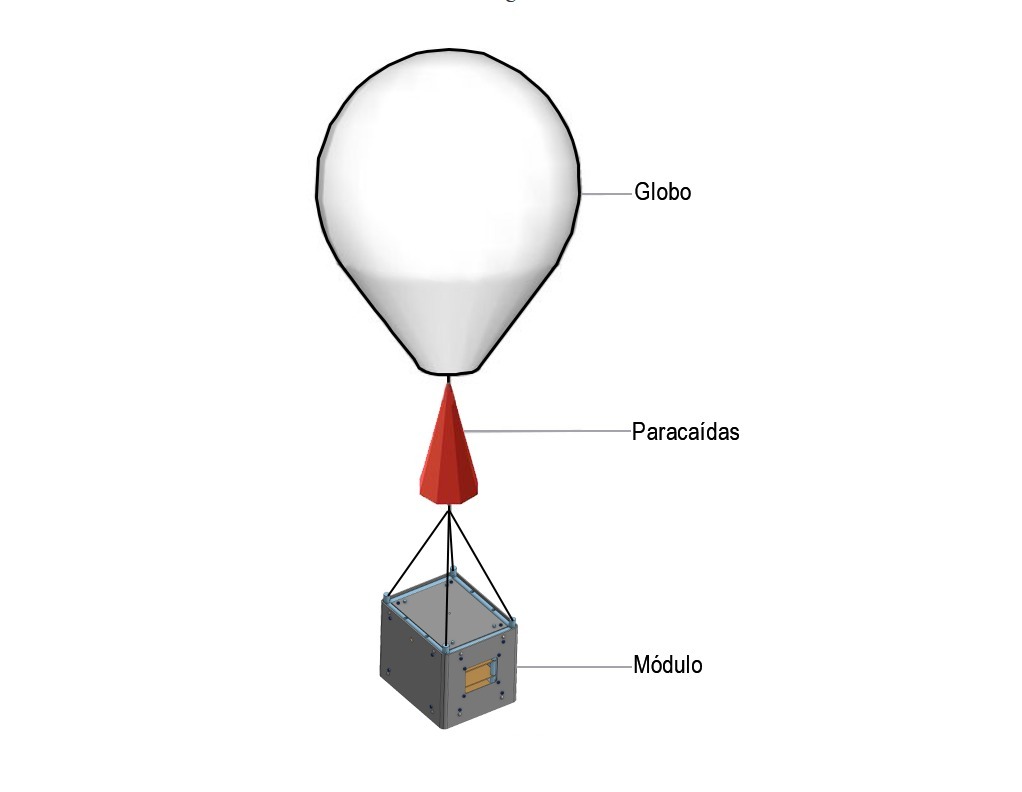
\includegraphics [width = 0.75\textwidth] {document/figures/01_componentes del globo}
    \caption{Bosquejo de StratoBalloon, créditos a \cite{tesis_estructura_stratoballoon}.}
    \label{fig:bosquejo_stratoballoon}
\end{figure}

\newpage

\subsection{Precedentes}

En el campo de la exploración espacial, en la última década se han desarrollado diversas plataformas open-source que han facilitado el  acceso y  democratizado la tecnología espacial como: 
 \begin{itemize}
     \item ArudPilot \footnote{ArduPilot Website: \url{https://ardupilot.org/}}.
     \item Dronecode \footnote{Dronecode foundation Website: \url{https://www.dronecode.org/}}
     \item Pycubed \footnote{Pycubed website: \url{https://pycubed.org/}}
     \item HabHub \footnote{HabHub website: \url{https://habhub.org/}}
 \end{itemize}

Las plataformas anteriormente listadas,  se ven principalmente impactadas en espacios académicos o por aficionados interesados en la exploración espacial, lo que contribuye a su crecimiento constante día a día. Existen y se pueden encontrar otras plataformas o precedentes a lo largo de internet, sin embargo, las plataformas que se mencionan a continuación  en subsubsecciones \ref{ssct:intro:pycuebed} y \ref{ssct:intro:habhub} han impactado significativamente el presente trabajo.

\newpage

\subsubsection{PyCubed} \label{ssct:intro:pycuebed}

Es un proyecto que desarrolla software y hardware en Python para  nanosatélites en estándar CubeSat, es apoyada por la Universidad de Stanford y dentro de sus recursos digitales se pueden encontrar las publicaciones realizadas, el código fuente, los diseños de las PCB's y diferentes misiones realizados con la iniciativa de este trabajo. Esta información  está habilitada en GitHub \footnote{Repositorio online: \url{https://github.com/pycubed}} o en su página web \footnote{Página Web: \url{https://pycubed.org/} }. 

La plataforma PyCubed, toma como ventaja que la electrónica embebida sigue en auge y en la última década ha existido una explosión importante, haciendo que el hardware se integra cada vez más y se utiliza ampliamente en todas las disciplinas de la ingeniería.  Esto se puede ver reflejado en las misiones KickSat-2 \cite{pycubed_kicksat-2}  y V-R3x \cite{pycubed_v-r3x} siendo avalados según sus propósitos de investigación por NASA.

En figura \ref{fig:ejemplo_pycubed}, se muestra una placa con características de bajo costo y la funcionalidad de integrar varios subsistemas (telemetría, navegación, energía, etc.) en una sola placa de circuito impreso.

\begin{figure}[!ht]
    \centering
    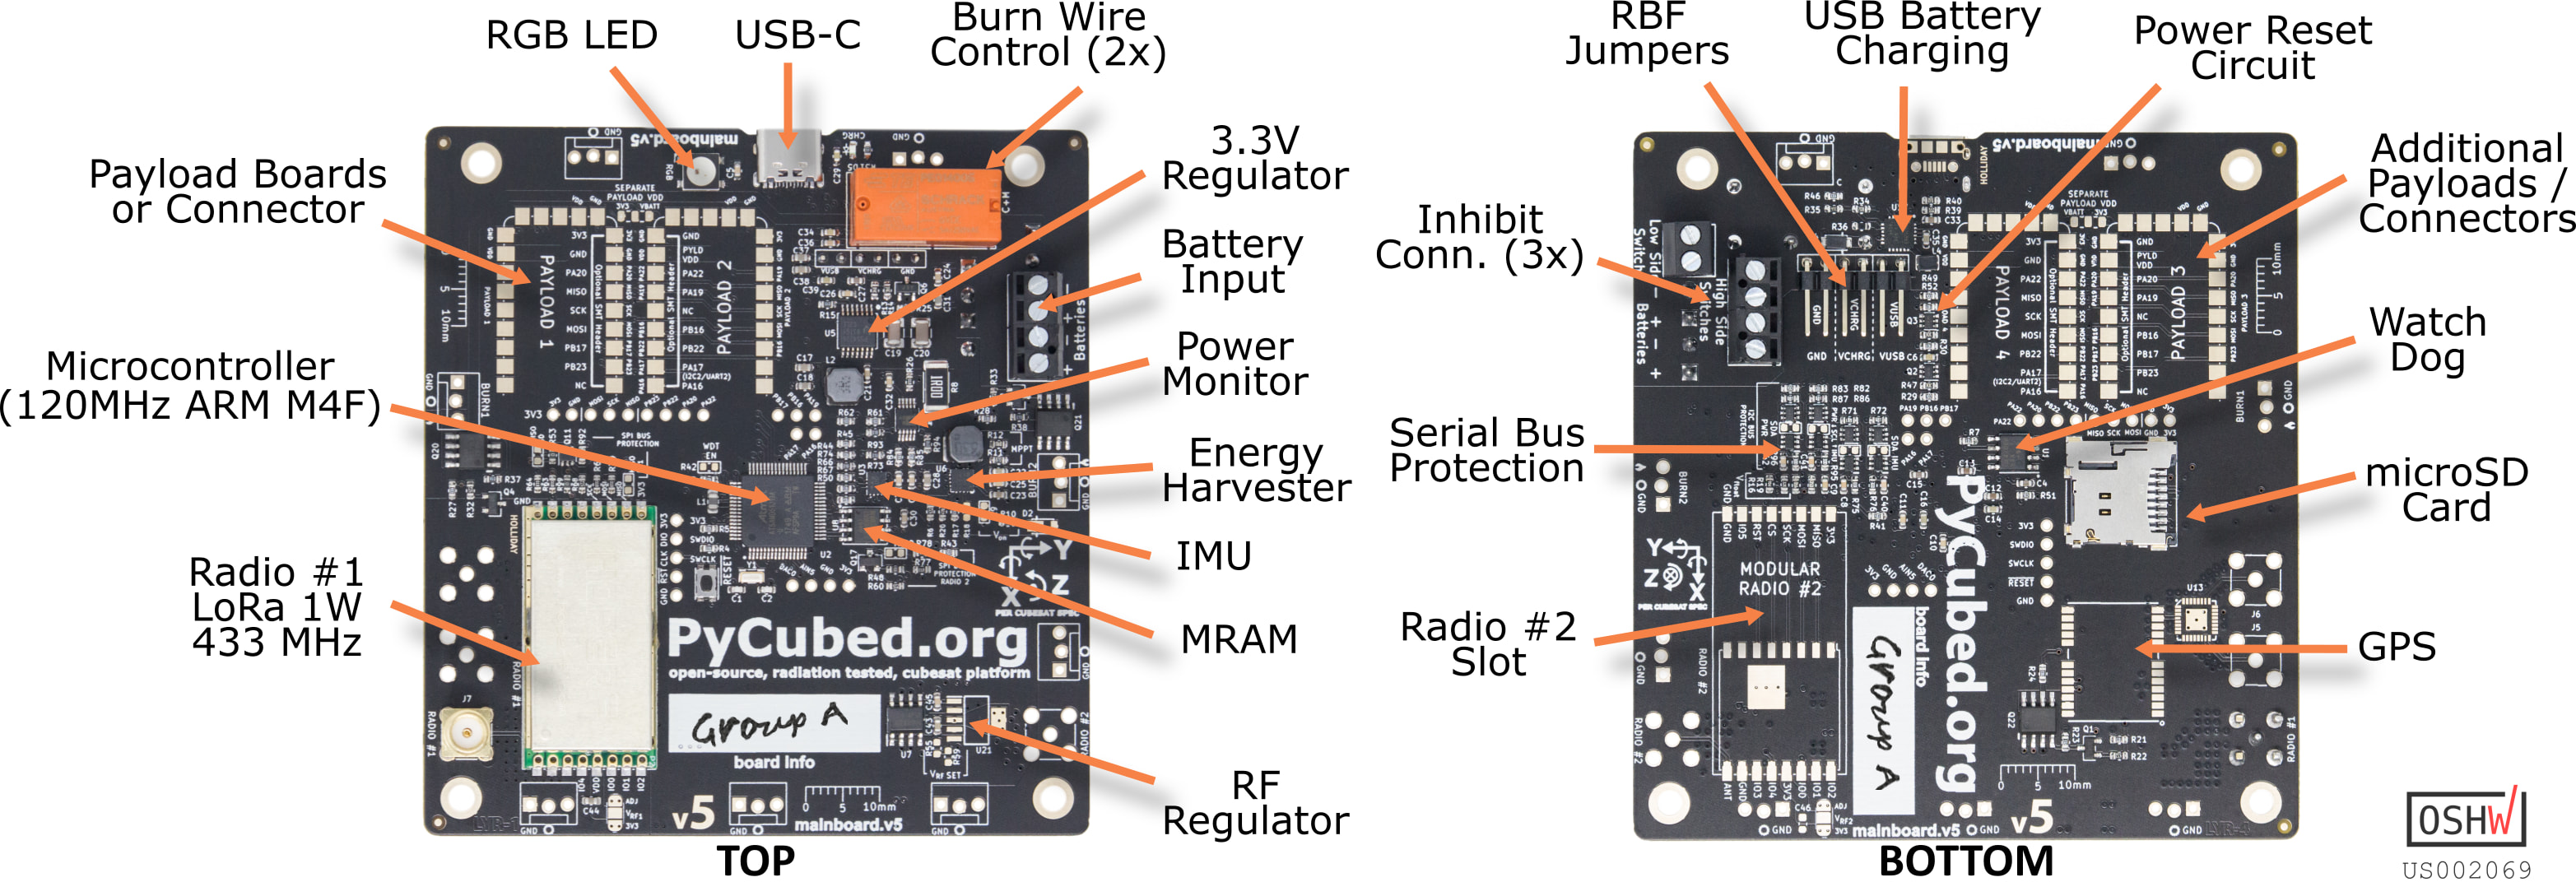
\includegraphics[width=0.75\linewidth]{document/figures/01_pycubed_ejemplo.jpg}
    \caption{PCB realizado por PyCubed, tomada de GitHub bajo CC BY-SA 4.0, sin modificación.}
    \label{fig:ejemplo_pycubed}
\end{figure}

\subsubsection{Habhub} \label{ssct:intro:habhub}

Es una plataforma dirigida por UK High Altitude Society (UKHAS)  que poseen múltiples herramientas en lo relacionado con globos de gran altitud, las cuales incluye: seguimiento y almacenamiento de los datos de vuelo, predicción de trayectoria y calculadora de explosión según la altitud. Además, incluye documentación y guías para montar un globo de forma aficionada\footnote{Página web:  \url{https://habhub.org/}}, ver figura \ref{fig:habhub}. 

\newpage

\begin{figure}[!ht]
    \centering
    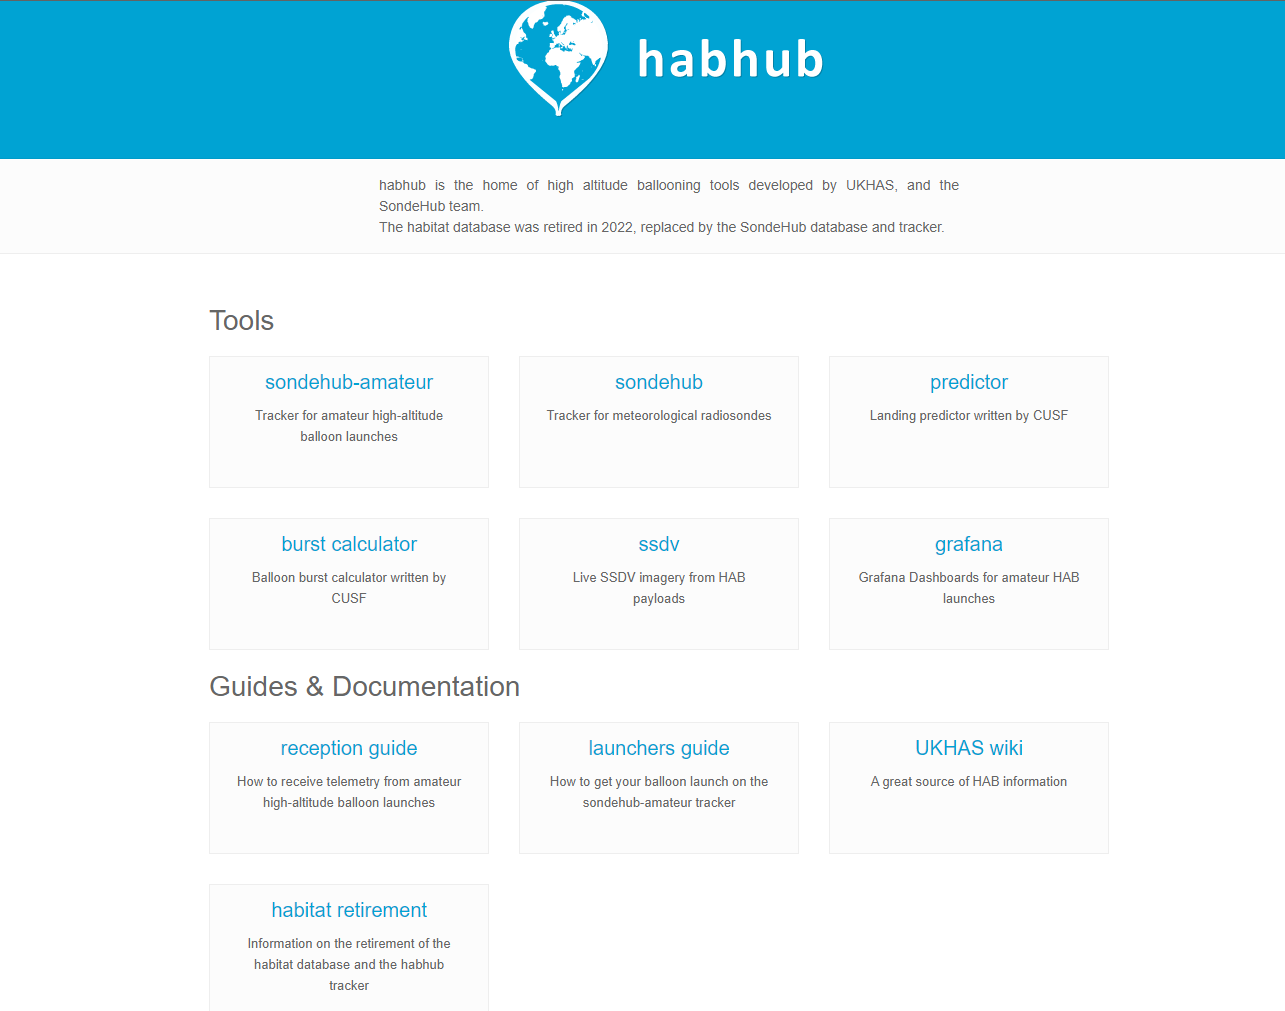
\includegraphics[width=0.5\linewidth]{document/figures/01_habhub_inicio.png}
    \caption{Inicio de la página web de habhub}
    \label{fig:habhub}
\end{figure}

Al visitar la página de HabHub y explorar las diferentes herramientas que ofrece (ver figura \ref{fig:cal_predic_habhub}), se encontró una calculadora útil para determinar la altitud de explosión de un globo de gran altitud. Esta calculadora recibe como parámetros de entrada el peso del payload, el tipo de globo, el objetivo de altitud o el objetivo de tasa de ascenso, y luego calcula la cantidad de gas de elevación (por defecto, se utiliza helio). Además, se encontró un software de predicción de ruta desarrollado por CUSF (Cambridge University Spaceflight) que acepta como parámetros la fecha, el lugar de lanzamiento, la altitud objetivo, entre otros (ver Figura \ref{fig:cal_predic_habhub}). El código fuente de la calculadora se puede consultar en internet\footnote{Calculadora: \url{https://github.com/projecthorus/cusf-burst-calc}} y el del software de predicción en\footnote{Software de predicción: \url{https://github.com/projecthorus/leaflet_predictor}}.

\begin{figure}[!ht]
    \centering
    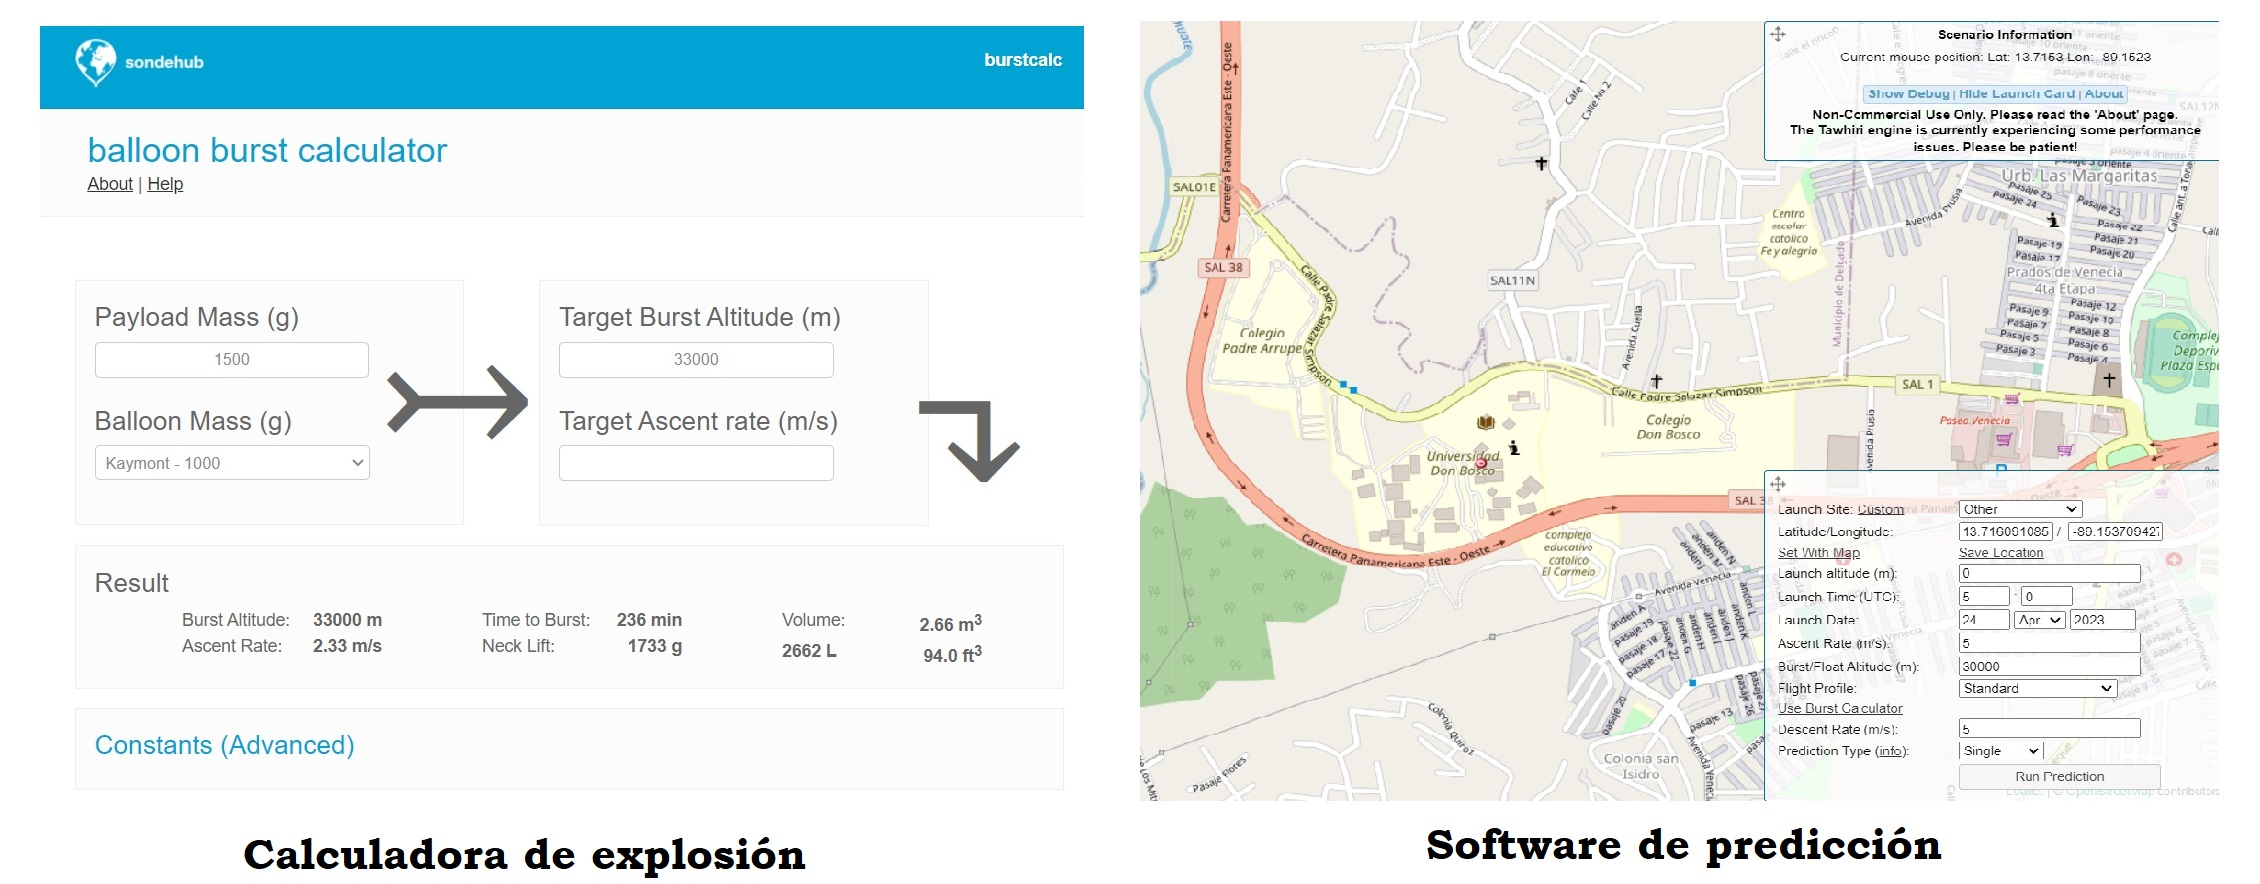
\includegraphics[width=0.95\linewidth]{document/figures/01_predic_calcBurst_habhub.jpg}
    \caption{Herramientas en su website, HabHub}
    \label{fig:cal_predic_habhub}
\end{figure}

\newpage

\subsection{Generalidades de los globos}

En lo que se refiere a la historia, ver figura \ref{fig:historia_globos},  se tiene registro del uso de globos en desde el siglo III en China se usaban como juguetes, fue hasta 1783 que los hermanos Montgolfier llenaron un globo de aire caliente llevando una persona en la ciudad París, Francia, los cuales ahora son llamados globos aerostáticos; y así fueron pasando los años se fueron realizando nuevos progresos haciendo que los globos lleguen más altos, se inventaron nuevos conceptos y tipos de globos hasta los de hoy en día \cite{history_type_balloon}.

\begin{figure}[!ht]
    \centering
    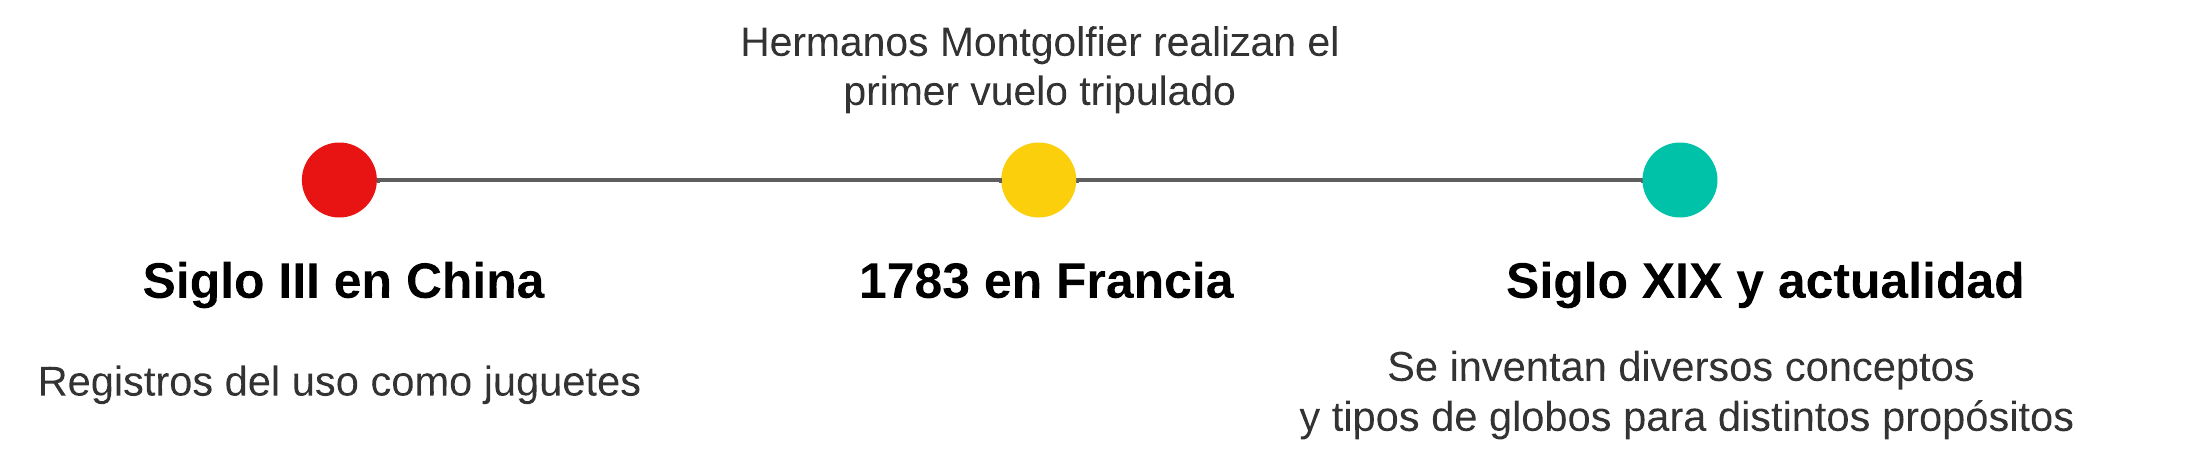
\includegraphics[width=0.5\linewidth]{document/figures/01_LineaTiempo_Globo_Historia.png}
    \caption{Evolución de los Globos a lo largo de la Historia}
    \label{fig:historia_globos}
\end{figure}

Los Globos de Gran Altitud (HAB), los cuales son vehículos semi espacial ligeros que transportan una carga y son capaces de sustentarse por medio de un gas como helio, nitrógeno, hidrógeno e incluso gas de carbón, ya que son menos densos que el aire. Estos vehículos obedecen al principio de Arquímedes en cuanto a la flotabilidad de un cuerpo y el peso aparente cuando están en otros fluidos, es decir, al diferenciar la densidad del vehículo con la densidad del aire y resulta que el peso aparente del vehículo es menor a cero, este será capaz de elevarse \cite{libro_fisica_giancoli}.

Un globo sonda está constituido generalmente por las siguientes componentes, que recuerda a figura \ref{fig:bosquejo_stratoballoon}:

\begin{itemize}
    \item \textbf{Globo:} Es la parte principal, el tipo de globo varía de acuerdo a la aplicación.
    \item \textbf{Paracaídas:} Una vez que el globo alcanza su altitud máxima, se hace necesario su descenso controlado y seguro para evitar daños en los equipos y garantizar la seguridad de las personas y propiedades en tierra.
    \item \textbf{Carga Útil:} Depende mucho del tipo de misión a realizar, sin embargo, algunos componentes comunes podrían ser: instrumentos científicos, sistema de comunicaciones y ubicación. 

\end{itemize}

\subsubsection{Tipos de Globos} \label{tipos_globo}

Los globos se pueden clasificar de muchas formas como podrían ser su aplicación, tipo de gas elevador, tripulados o no tripulados, uso civil, científico o militar, etc. Sin embargo, los globos sonda de gran altitud, los cuales son el interés para este trabajo,  se clasifican como indica \cite{type_balloon_NASA, history_type_balloon, just_type_balloon} de esta forma:  

\begin{itemize}
    \item \textbf{Sounding Balloon or Weather Balloon}: en español se conocen como globos meteorológicos, son típicamente fabricados en látex y son diseñados para expandirse y explotar a una altura determinada, recolectando datos en su ascenso, sin superar la estratosfera.  Existe una variedad de nombres tanto en inglés como en español para este tipo de globo, así como una diversidad de aplicaciones y usos según el contexto. Principalmente, se observa su uso en universidades y centros de investigación. 
    \item \textbf{Equal pressure or Zero-pressure Balloons}: Los globos aerostáticos de igual presión o presión cero transportan cargas útiles a grandes altitudes en la atmósfera terrestre. Se diferencian de los globos de gas convencionales en que se llenan de helio a temperatura ambiente y se dejan expandir de forma natural a medida que ascienden, en lugar de inflarlos con gas a presión. Al incorporar una bolsa de lastre o un sistema de válvulas que libera gas cuando la presión dentro del globo aumenta debido al ascenso de este, los globos mantienen su forma.
    \item \textbf{Super Pressure Balloons}: conocidos en español como "globos de superpresión" mantienen una altitud y una forma constantes al mantener una sobrepresión continua dentro de la envoltura del globo. Se utilizan para la investigación científica. Pueden transportar cargas más pesadas durante períodos más largos que otras variedades de globos aerostáticos porque no les afectan las variaciones de la presión atmosférica. Su tamaño y peso, que dificultan su lanzamiento y recuperación.
\end{itemize}

A continuación, se muestra en figura \ref{fig:type_balloons} los tipos de globos ordenados según se listaron anteriormente. Créditos a las imágenes a \footnote{NASA/Bill White. Ver en: \url{https://www.flickr.com/photos/nasakennedy/36612463502}} \footnote{NASA. Ver en: \url{https://www.flickr.com/photos/nasafo/48877773637}} \footnote{NASA/Bill R. En: \url{https://www.flickr.com/photos/nasakennedy/36612463502}}, tomadas de Flickr.

\begin{figure}[!ht]
    \centering
    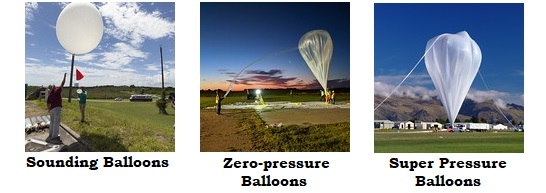
\includegraphics[width=0.9\linewidth]{document/figures/01_type_ballons.jpg}
    \caption{Tipo de globos de gran altitud}
    \label{fig:type_balloons}
\end{figure}

